\begin{figure}[t]
 \centering
  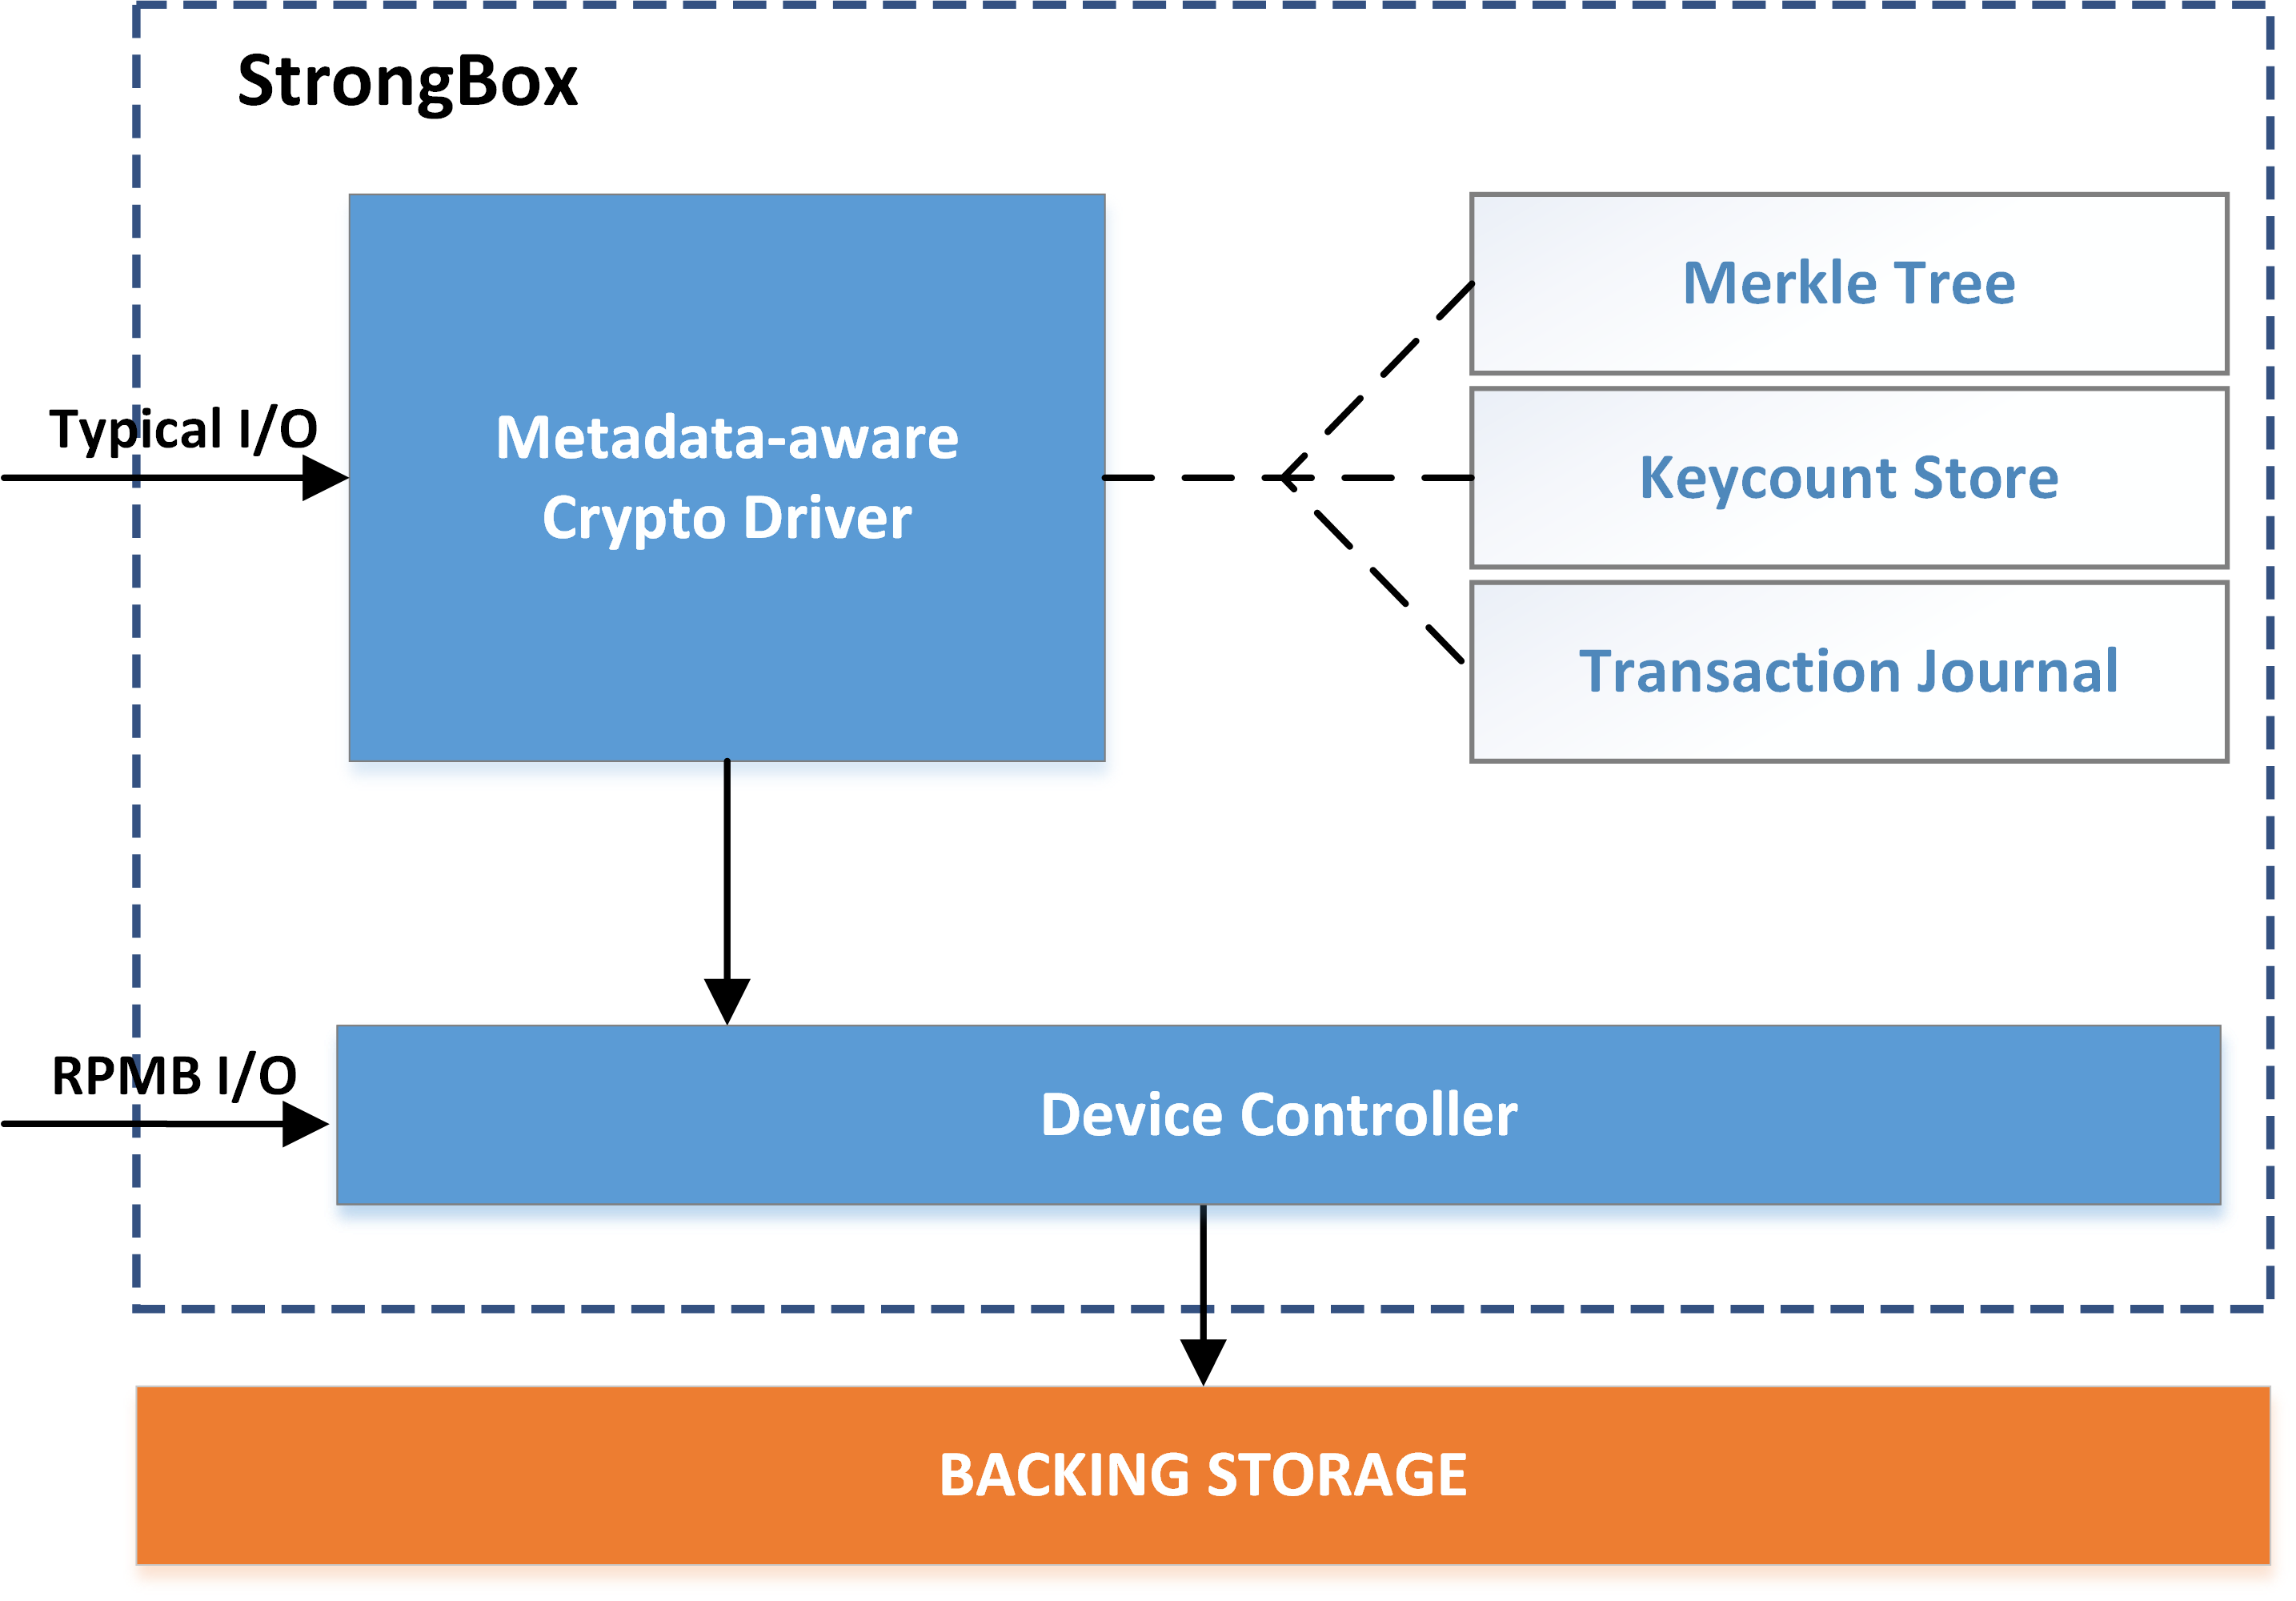
\includegraphics[width=\linewidth]{overview.png}
   \caption{Overview of the \SYSTEM{} construction.}\label{fig:overview}
\end{figure}

\section{\SYSTEM{} Design}\label{sec:design}

\TODO{How much of the original StrongBox should be explained here? Is this too
much? Too little?} \TODO{Hank: This is a good overview.  Right now, the level of
detail feels right to me. There are two things missing, however.  First, we need
a clear delineation between prior work and this paper.  One way to make that
distinction is to point at the diagram and say this piece is new.  Another way
would be if it is a conceptual difference.  I believe this case is a combination
of both: (1) there is at least some new metadata to be added (to accomodate
freestyle IIRC) plus I would assume that StrongBox does not include a field for
cipher in the nugget and (2) there is the conceptual change that now each nugget
can have a different scheme (not just key). Second thing that is missing: need
to talk about what is coming in the section.  This second thing should relate to
the first, as we should spend most of the time talking about what is new for
this paper.}

\SYSTEM{}, like StrongBox and Adiantum, is a translation layer positioned
between the block layer and the operating system's virtual file
system~\cite{StrongBox,Adiantum}. There are several places \SYSTEM{} could be implemented
in the system stack: as part of an actual kernel Log-structured File System
(LFS) module like the F2FS filesystem, as a block device or virtual block device
in the manner of dm-crypt, or within a device controller such as an SSD drive
controller's FTL~\cite{StrongBox}.

\figref{overview} illustrates the \SYSTEM{} design. \SYSTEM{} manages five
metadata components: an in-memory \emph{Merkle Tree}; two drive-backed byte
arrays, \ie{the \emph{Keycount Store} and the \emph{Transaction Journal}}; a
globally persistent cryptographically secure monotonic counter; and a flexible
drive-backed store for per-nugget cipher-specific metadata. For our monotonic
counter implementation, we used a \emph{Replay Protected Memory Block} (RPMB).
\TODO{Citation would be good here.  But, it is a little strange to get so
specific in this part of the text.  I would either save it for a later
implementation section (or evaluation).  Or, if you think that the existence of
these counters might be controversial, then say we use RPMB, but we could have
used many others such as...}

These five components are tightly integrated into the cryptographic driver,
which handles data encryption, decryption, overwrite detection, integrity
protection, communication with the wider system to determine the active cipher,
and the application of cipher switching strategies. The cryptographic driver
interacts with 1) the overlying LFS through traditional I/O passed through the
Linux Virtual Filesystem Switch (VFS) as well as 2) the underlying backing store
through the device controller block I/O layer.

\SYSTEM{} uses IPC to receive commands to toggle the active cipher between the
primary and secondary ciphers. \TODO{Spell out the acronym the first time it is
used.}

\begin{figure}[t]
 \centering
  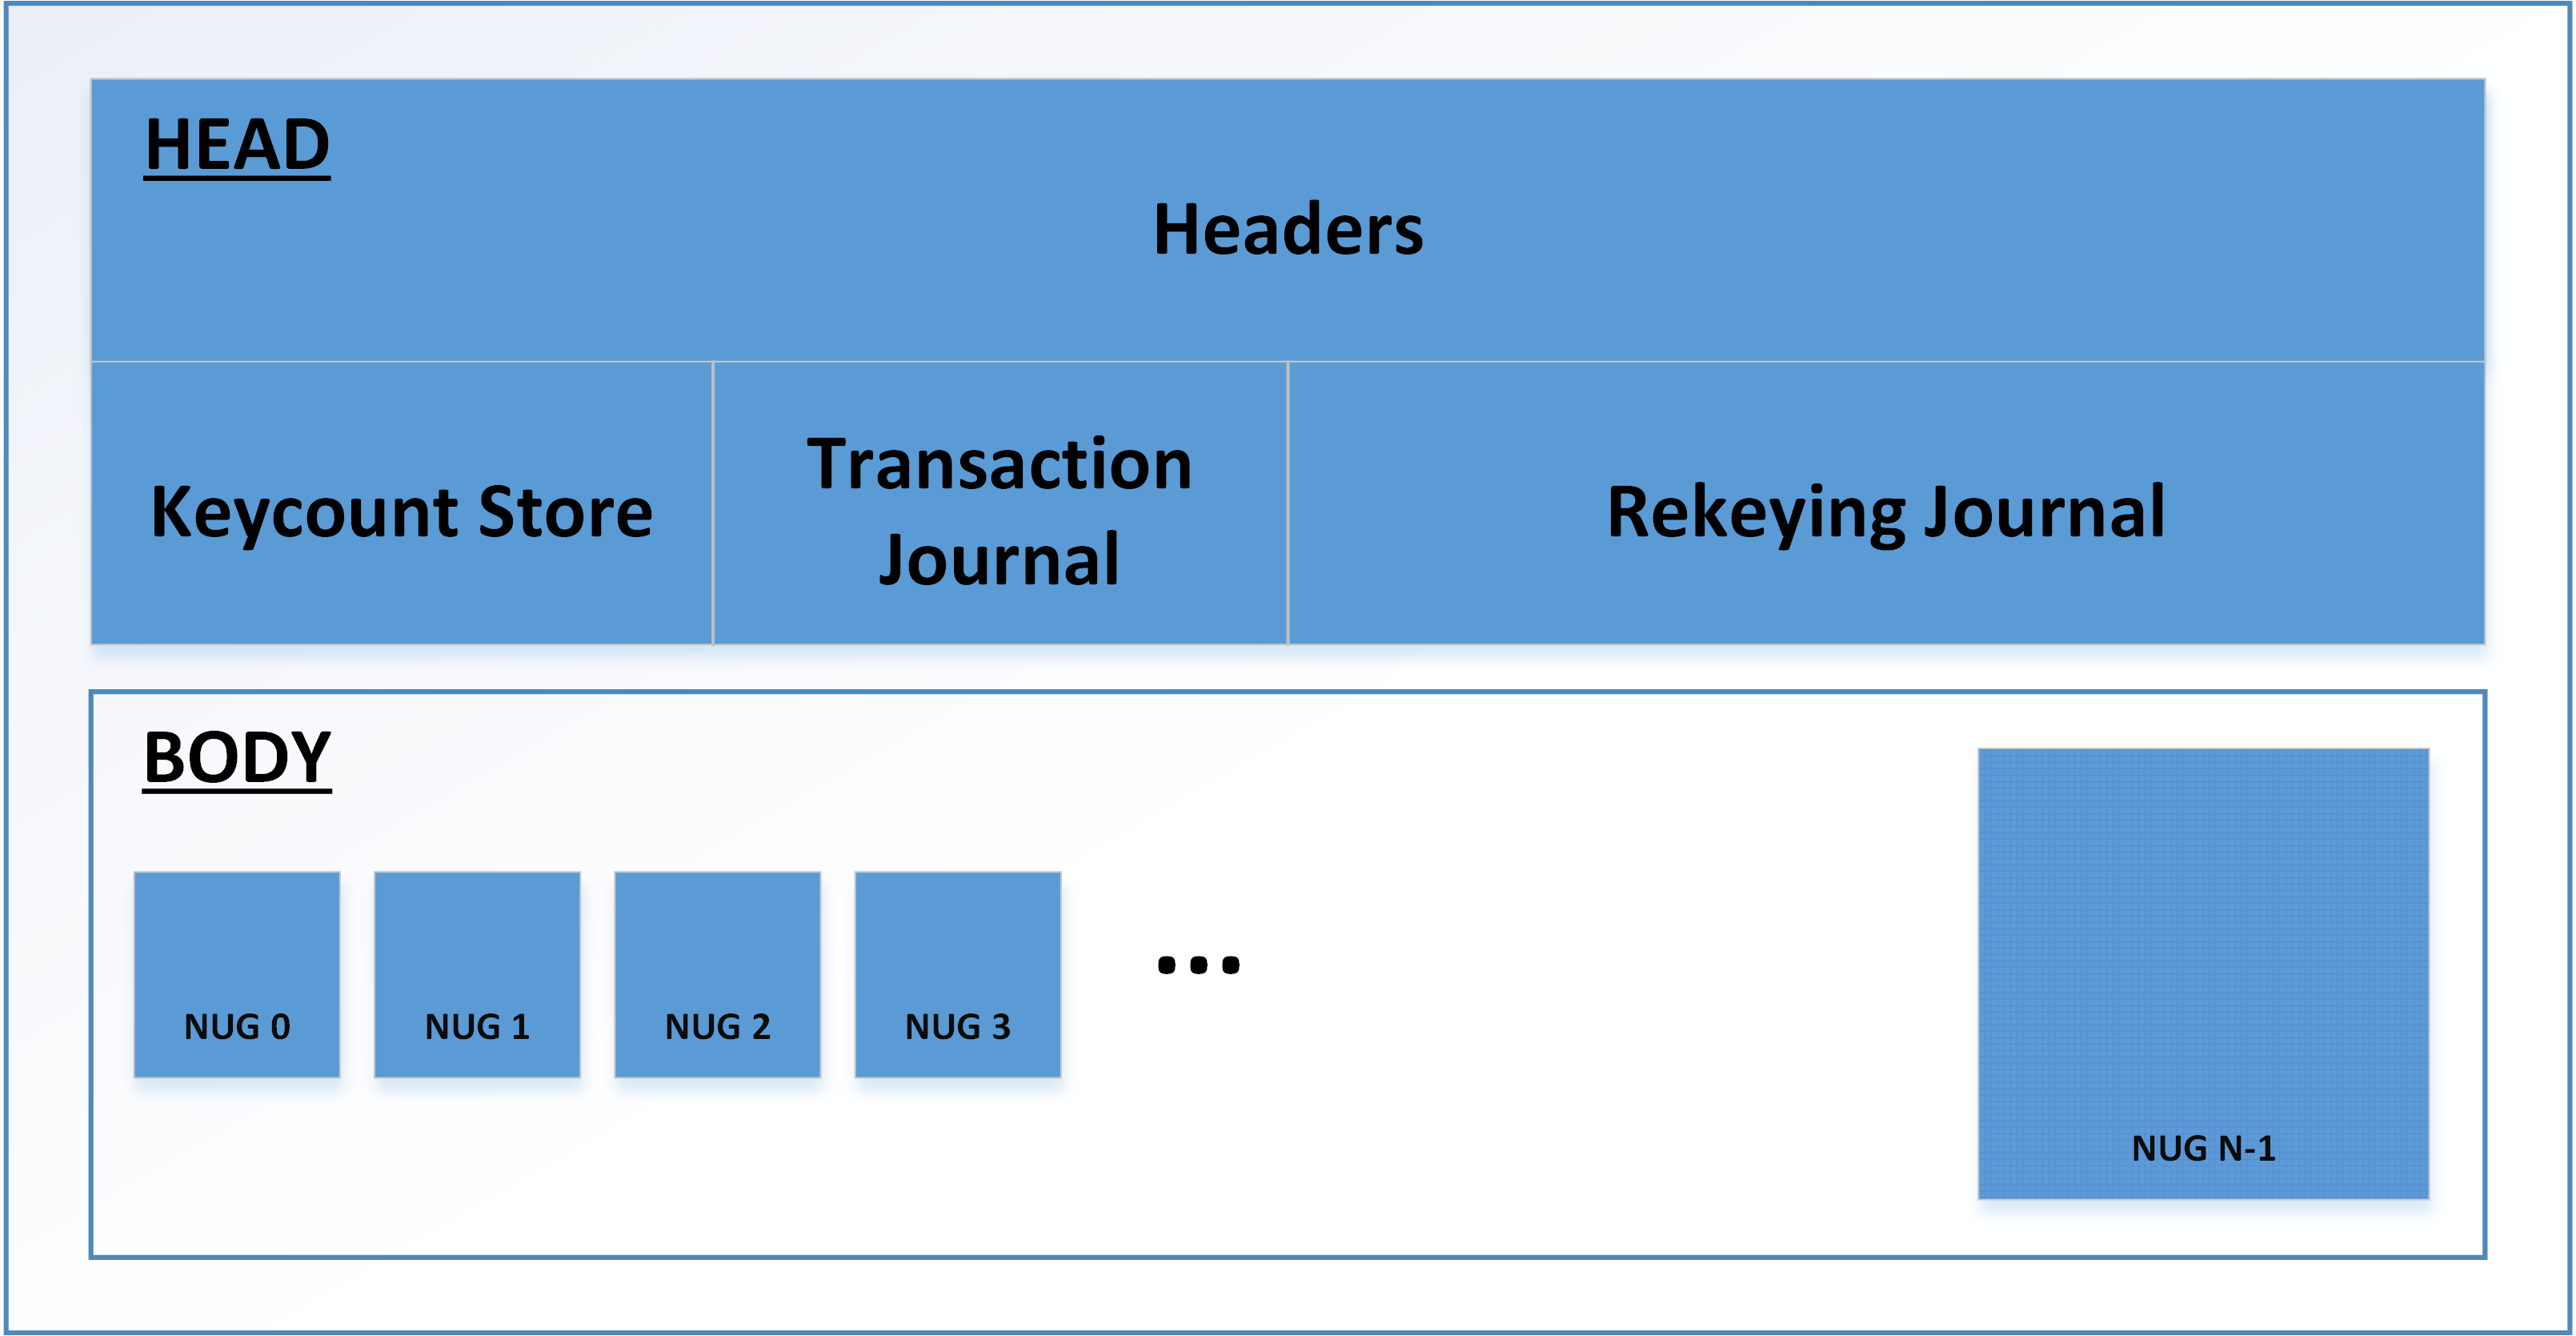
\includegraphics[width=\linewidth]{backstore.png}
   \caption{Layout of \SYSTEM{}'s backing storage.}\label{fig:backstore}
\end{figure}

The backing store is the storage medium \SYSTEM{} operates on. The layout of the
backing store is illustrated in \figref{backstore}. In the \textit{body} section
of the backing store layout, end-user data is partitioned into a series of
same-size \emph{logical blocks}---which are distinct from the concept of
\emph{physical drive blocks}---we refer to these wider logical blocks as
\emph{nuggets}, marked \textit{NUG}. Hence, a nugget consists of one or more
physical drive blocks along with per-nugget metadata indicating if the nugget
was encrypted with the primary or the secondary cipher. \TODO{Do we redescribe
the rest of the backing store from StrongBox, or should we link to the original
paper? Or should we skip talking about the backing store at all and more briefly
describe nuggets here? It's all not very different from StrongBox's, i.e. an
extra header was added.}

In the rest of this section, we describe our cipher switching strategies. We
also discuss the pluggable stream cipher API and other design challenges. This
is followed by an explanation of implementation-specific details and a
discussion of the overall implications and limitations of \SYSTEM{}'s design.

\subsection{Cipher Switching Strategies}

Upon initialization, prior work requires a single cipher to be selected. The
specified cipher---ideally along the pareto frontier of security and energy
tradeoffs---is then used to encrypt and decrypt all data on the filesystem. With
\SYSTEM{}, however, \emph{a pair of ciphers are selected} upon initialization,
depending on the concerns of the end-user. These ciphers are referred to as the
\emph{primary cipher} and the \emph{secondary cipher} respectively, and
represent the static configuration points along the pareto frontier between
which \SYSTEM{} can navigate. \TODO{Do you really have to know these ahead of
time? If I had a cipher API and managed the implementation as a DLL, could I
switch to any cipher, by just building a new DLL? Is there any reason, you
couldn't have three or four or N ciphers and switch between all of them?  I ask
all these questions because I want you to separate the conceptual idea, which
should be as broad as possible, from the specific choices you had to make to
demonstrate the idea (which may be much more restricted).  Here we want to
discuss the conceptual ideas and save details for the implementation.}

At any moment, the currently active cipher is used to interact with the backing
store. Initially, the primary cipher is the active cipher. Until the wider
system indicates that \SYSTEM{} should use a different cipher to interact with
the backing store, \SYSTEM{} functions identically to StrongBox in that it uses
the primary cipher to encrypt and decrypt all nuggets during I/O.

However, switching the active cipher dynamically allows \SYSTEM{} to achieve
optimal configuration points that are otherwise unachievable with prior work.
The wider system determines if the primary or secondary cipher should be the
active cipher at any given moment, and \SYSTEM{} responds immediately.
Unfortunately, it is entirely non-trivial to determine \emph{when} to re-encrypt
a nugget with a different cipher and \emph{where} to direct the output of that
cipher. \TODO{Don't just say it is difficult, make an argument about why it is
difficult.  It is often very helpful to say things that are obvious to you
because they won't be obvious to the reader, but will help build intuition for
what is coming.  For example, you can say that one simple approach would
immediately convert the entire drive, but the cost of doing that conversion
might consume more energy than would be saved in future accesses.  I do like
using where and when to set up spatial and temporal switching.  }

Hence, cipher switching \emph{strategies} are the mechanism by which \SYSTEM{}
can effectively transition nuggets between different encrypted states
dynamically, thus providing a mechanism to navigate the tradeoff space presented
in \figref{40mb-read-with-forward}. \TODO{Expound on this all more? Reword?
Delete? Different chart referenced here instead?} \TODO{Hank: expound! Go ahead
and say that when to target the new encryption is temporal switching and we
propose a specific strategy, \emph{Forward}, to handle it.  Where to switch is
spatial switching and we propose two strategies to deal with that.}

\subsubsection{Forward}

\SYSTEM{} allows each individual nugget to exist encrypted using one cipher or
the other regardless of the currently active cipher. When a nugget is
encountered during I/O that is encrypted using a cipher other than the active
cipher, however, the forward strategy dictates that this nugget be re-encrypted
"just-in-time" using the active cipher before completing the I/O operation. If a
particular nugget encrypted with the non-active cipher is never encountered
during I/O, it is never re-encrypted and remains on the backing store in its
original state. In this way, the forward strategy represents a form of temporal
cipher switching.

Rather than re-encrypt the entire backing store every time the active cipher
changes, this strategy limits the performance impact of cipher switching to
individual nuggets. Similar to rekeying in the original StrongBox construction,
the heavy price of re-encryption is paid only once during the initial
re-encryption, after which the nugget is accessed normally during I/O until the
active cipher is switched again.

There are several forms the forward strategy can take. The default and most
intuitive is \emph{0-forward}, in which \SYSTEM{} immediately transitions
individual nuggets encountered during I/O to the active cipher is they are not
using it. Over time, if various I/O operations end up touching every nugget in
the backing store, the encrypted state of every nugget will eventually become
consistent with the currently active cipher.

The forward strategy can also take the form of \emph{N-forward}, where \SYSTEM{}
attempts to take advantage of spatial sequential locality to transition whole
sets of nuggets into the active cipher. We can trivially expand the forward
strategy to encompass the entire backing store by selecting N equal to the total
number of nuggets managed by \SYSTEM{}. This would have the overhead of
re-encrypting large swaths of the backing store upon every I/O operation where a
nugget encrypted with the non-active cipher is encountered. Of course, this has
the same effect as simply re-initializing the entire filesystem with the new
cipher.

\subsubsection{Selective}

When \SYSTEM{} is initialized with the selective strategy, the backing store is
partitioned into two regions governed exclusively by the primary and secondary
ciphers, respectively. All nuggets in the first partition are encrypted with the
primary cipher while all nuggets in the second partition are encrypted with the
secondary cipher.

Hence, unlike the forward strategy, which schedules individual nuggets to be
re-encrypted at some point in time \emph{after} the active cipher is switched,
the selective strategy allows the wider system to indicate \emph{where} on the
backing store a read or write operation should occur: either in one partition or
the other. In this way, the selective strategy represents a form of spatial
cipher switching where different regions of the backing store can store
different pieces of data.

\subsubsection{Mirrored}

Similar to the selective strategy, when \SYSTEM{} is initialized with the
mirrored strategy, the backing store is partitioned into two regions governed
exclusively by the primary and secondary ciphers, respectively. All nuggets in
the first partition are encrypted with the primary cipher while all nuggets in
the second partition are encrypted with the secondary cipher.

However, unlike the selective strategy, all write operations that hit one
partition are mirrored into the other partition immediately. The mirrored
strategy allows the wider system to indicate where on the backing store a
\emph{read} operation should occur. As a result, both regions of the backing
store will always be in a consistent state and share the same data. In this way,
the mirrored strategy, like the selective strategy, represents a form of spatial
cipher switching.

\subsection{Pluggable Stream Cipher API}

\TODO{Always use present tense in technical writing.  It should be we develop
instead of we developed.} We developed an API to allow any stream cipher or any
cipher that can pose as a stream cipher to be used with \SYSTEM{} without
modification, including ciphers with residual output, \eg{Freestyle}. \TODO{I
don't know what residual output is, so please expand on the differences between
ciphers that causes problems. But before you do, see the note below on
challenges.} \SYSTEM{} exposes a common encryption and decryption interface,
including read and write handles, that allow \SYSTEM{} to transition nuggets
between arbitrary ciphers at the behest of the wider system. \TODO{This section
is odd here.  Having a whole subsection seems to imply that it is as important
as the switching strategies, but having a short paragraph implies it is more of
a side note.  In addition, it is not clear what purpose this discussion serves.
I think you need more setup about how different stream ciphers might appear to
all be interchangeable, but they are not, so we need a common interface---again,
sometimes it is actually helpful to state what feels obvious to you.}

\subsection{Challenge: Beware Naive Forward Switching}

It is tempting to implement forward switching such that a nugget is re-encrypted
during I/O if its metadata indicates that it was previously encrypted using the
non-active cipher. However, such a naive implementation can have disastrous
effects on performance depending on the workload.

First, a nugget is considered "pristine" if it has not had any data written into
it yet. \SYSTEM{} determines if a nugget is pristine by checking the state of
the transaction journal for that nugget. A pristine nugget will have a clean
transaction journal.

All nuggets start out as pristine. All nuggets start out with metadata
indicating that they're to be encrypted and decrypted by the primary cipher
(which is the initially active cipher when \SYSTEM{} is first initialized). This
is true \emph{even if the nugget has not been written to yet}. This means, on
read and write operations after the secondary cipher becomes the active cipher
using a naively implemented forward switching strategy, every write operation
will trigger a re-keying, which carries significant overhead.

The solution is to divide forward switching into \emph{soft re-encryption} and
\emph{hard re-encryption}. Fortunately, the \SYSTEM{} design lends itself nicely
to such a distinction for free, as per-nugget metadata is managed separately
from a nugget's actual data.

During soft re-encryption, only the nugget's metadata is changed to indicate
that the nugget can be encrypted and decrypted with the newly active cipher but
\emph{without actually re-encrypting the nugget data itself}. This keeps the
nugget in a "pristine" condition, preserving \SYSTEM{}'s ability to write data
into it without triggering a costly rekeying operation every time, preserving
the original StrongBox's performance advantage. At the same time, \SYSTEM{} can
now use the newly active cipher to interact with the nugget as expected.

On the other hand, during hard re-encryption, the nugget's metadata is changed
to match the active cipher \emph{and} the nugget data is re-encrypted using the
new cipher. When using forward switching other that 0-forward, \ie{N-forward}
where $N > 0$, only read operations are allowed to trigger hard re-encryption
for nuggets other than the currently active nugget. This is still not enough to
preserve StrongBox's performance advantage, however, as I/O operations can span
multiple nuggets, and attempting to take advantage of spatial locality after
interacting with every nugget is counterproductive. Hence, only the last nugget
touched by a read or write operation will trigger the more aggressive N-forward
behavior if $N > 0$.

These considerations have the effect of 1) preserving the original StrongBox
performance advantage over prior work and 2) allowing more aggressive N-forward
behavior (where $N > 0$) to take advantage of spatial locality during read-heavy
workloads to result in a further performance advantage (c.f.
\secref{evaluation}).

\TODO{Note: Hank wrote the followign before the Challenge section was updated,
some of it is still relevant.  Earlier text: Are the challenges really just
overhead?  I think there are a couple of other challenges, like: when to switch?
Which blocks to switch?  How to make ChaCha type ciphers work with Freestyle
type ciphers?  Basically, every piece of the system that you think is
interesting is probably interesting because it addresses some challenge.  For
that reason, I think this section should be moved earlier, as it should be a
discussion of the challenges that need to be overcome by the design.  So, the
flow would be overview (what we want to do), challenges (why it is hard),
description of key components (with references to how they help us accomplish
the overall goal and how they address the challenges), then implementation (how
do we go from the conceptual design to a working system)}.

\subsection{Implementation}

Our \SYSTEM{} implementation consists of 9,491 lines of C code; our test suite
consists of 6,077 lines of C code. All together, our solution is comprised of
15,568 lines of C code.

\SYSTEM{} uses OpenSSL version 1.1.0h and LibSodium version 1.0.12 for its
AES-XTS and AES-CTR implementations. Open source ARM NEON optimized
implementations of ChaCha are provided by Floodyberry~\cite{Floodyberry}. The
Freestyle cipher reference implementation is from the original Freestyle
paper~\cite{Freestyle}. The eSTREAM Profile 1 cipher implementations are from
the open source libestream cryptographic library~\cite{libestream} by Lucas
Clemente Vella. As with the original StrongBox construction, the Merkle Tree
implementation is from the Secure Block Device~\cite{SBD}. \SYSTEM{}
implementation is publicly available open-source\footnote{\SystemURI}.

For a fair comparison with the original StrongBox implementation, we mirror
their use of the BUSE~\cite{BUSE} virtual block device as our device controller.
BUSE is a thin (200 LoC) wrapper around the standard Linux Network Block Device
(NBD). BUSE allows an operating system to transact block I/O requests to and
from virtual block devices exposed via domain socket.

For the purposes of our implementation, we make the choice of ciphers binary:
either the system wants \SYSTEM{} to access the backing store using the primary
cipher or the secondary cipher. However, there is no technical limitation
preventing various different nuggets encrypted with three, four, or more unique
ciphers from co-existing on the backing store. \TODO{Good detail.  In this case,
remove the discussion above about how we just support two ciphers.}

\subsubsection{Indicating a Cipher Switch Should Occur}
\TODO{As a style thing, you should avoid a subsub (or any breakdown) if there is
only one piece.  Usually a section with only one subsection indicates that there
is some organizational problem in the document. Update: I wrote this before I
merged with the new design section.  Now it is not relevant to this text, but I
will leave it here as general advice.  Just comment it out after reading. }

When \SYSTEM{} should be using the primary cipher or the secondary cipher to
interact with the backing store, this intent is communicated via POSIX message
queue in our implementation. It is not a requirement of \SYSTEM{} that a POSIX
message queue be used over any other method of inter-process communication (IPC)
so long as \SYSTEM{} is notified asynchronously when the wider system desires
one cipher be active over the other. \TODO{I am not sure why this section is
here.  It is either too much detail, or more likely there is some important
issue, but whatever that is needs to be stated much more explicitly.  Like maybe
the problem is that the user needs to actually communicate with the \SYSTEM{}
implementation and we need a mechanism to do that?  Anyway, assuming you expand
this a little so it is clear what problem is being addressed, then you can just
make this another paragraph in implementation instead of splitting it out into a
subsub.}

\TODO{I think the discussion here only covers temporal switching.  I believe you
should indicate that for this paragraph and then have a second paragraph that
talks about how to indicate that a spatial switch should occur (and you might
need a different method for mirrored and selective).  Correct me if I am wrong,
but I believe that the selective switch will require the IOp to indicate that
this data needs to be handled in one way or another.}

\subsubsection{Backing Store Initialization}

To operate securely, \SYSTEM{} must be seeded with random data initially rather
than have the backing store consist of all zeroes. This is a one-time cost paid
during initialization and has no tangible effect on performance.

If nuggets are not seeded with random data initially, any write operation into
an "empty" nugget might leak information or constitute an overwrite where the
predictable state of the backing store (\ie{initialized to all zeroes}) leads to
an overwrite-style condition.

%\subsection{Discussion}
% Should this be saved for the evaluation section? Should some of the other
% parts of this section be broken off into a discussion subsection?

\subsection{Discussion}
% Should this be saved for the evaluation section?
\TODO{You should include a discussion here if it is a conceptual discussion, for
example about the benefits and limitations of the proposed design.}

\TODO{Hank: I have one major issue at this point in the document.  I don't think
we should wait until discussion to address it, but I am writing about it here
because it was not addressed anywhere else.  I feel like we need some discussion
of threat model or something.  For example, I really like the mirroring
strategy, but I think it breaks if an attacker has physical access to the drive,
right?  Like if they have to request IO through the OS, I think it works becuase
the os or hypervisor can hide the mirrored side, but you can't hide that if I
can just read bytes off the drive itself, right?  Sort of similar for forward.
We really do need to say something about when these are applicable and when they
aren't.}\TODO{Bernard: Agreed (here and in your email)! We definitely need a
threat model subsection somewhere. The way I've been conceptualizing it is: the
OS can quickly kill half of the mirrored strategy with TRIM. But otherwise, yes,
the data will exist in both forms.}
